\documentclass{scrartcl}
\usepackage{pgfplots}
\usepackage{graphicx}
\usepackage{amssymb}
\usepackage[left=1cm, right=1cm, top=1cm, bottom=3cm]{geometry}

\usepackage{titlesec}
\titlelabel{\thetitle)\quad}

\begin{document}

	\title{\vspace{-2cm}Compte-rendu de travaux pratiques de physique}
	\subtitle{Régimes transitoires}
	\author{Benjamin LOISON et Lucas BOISTAY (MPSI 1)}
	\date{}
	\maketitle

	\section{Circuits soumis à des échelons de tension}

		\subsection{Circuit de type RC}
		
			\subsubsection{Observer qualitativement l'influence de la valeur de R et de C sur les courbes de charge et de décharge}
			
				En faisant varier la résistance du système, on constate que la charge diminue, tandis que faire varier le condensateur n'influe pas sur la tension.
				%On remarque que R et C influent sur la forme de la courbe.% best ?
				
			\subsubsection{On se propose d'étudier plus particulièrement la charge du condensateur}
			
				%On considère que ln signifie la fonction logarithme en base 10.\\
			
				\begin{tabular}{|c|c|c|c|}% sure dimension t and i ? and more values ?
					\hline t (en $\mu$s) & i (en mA) & ln(i) (avec i en mA))& U (en V)\\
					%\hline 250 & -3.12\\
					%\hline 500 & -960 * 10$^{-3}$\\
					%\hline 750 & -312 * 10$^{-3}$\\
					\hline 34 & 12.1 & 2.49 & 11.67\\ % 2.49 (ln) % 1.08 (log)
					\hline 48 & 10.3 & 2.33 & 10.34\\ % 2.33 % 1.01
					\hline 76 & 8.14 & 2.10 & 8.14\\ % 2.10 % 0.91
					\hline 112 & 5.96 & 1.79 & 5.96\\ % 1.79 % 0.78
					\hline 156 & 3.96 & 1.38 & 3.96\\ % 1.38 % 0.60
					\hline 192 & 3.01 & 1.10 & 3.01\\ % 1.10 % 0.48
					\hline 246 & 1.81 & 0.59 & 1.81\\ % 0.59 % 0.26
					\hline 290 & 1.30 & 0.26 & 1.30\\ % 0.26 % 0.11
					\hline
				\end{tabular}\\\\
			
			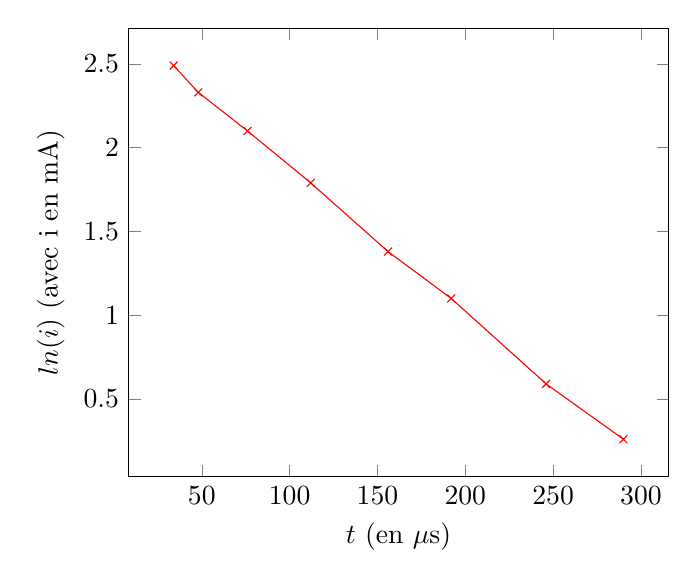
\begin{tikzpicture}
			\begin{axis}[
				xlabel=$t$ (en $\mu$s),
				ylabel=$ln(i)$ (avec i en mA)]
			\addplot[color = red, mark = x] coordinates {
				%(250, 0.494) % here log
				%(500, -0.0177)
				%(750, -0.506)
				
				%(34, 1.08)
				%(48, 1.01)
				%(76, 0.91)
				%(112, 0.78)
				%(156, 0.60)
				%(192, 0.48)
				%(246, 0.26)
				%(290, 0.11)
				
				(34, 2.49)
				(48, 2.33)
				(76, 2.10)
				(112, 1.79)
				(156, 1.38)
				(192, 1.10)
				(246, 0.59)
				(290, 0.26)
			};
			\end{axis}
		\end{tikzpicture}
			
			D'après la loi d'Ohm, on a: $I = \frac{U}{R}$, or $R$ = 1 k$\Omega$ donc $I = \frac{U}{1000}$.\\
			On a la relation: $i(t) = i_0 * exp\left(\frac{-t}{\tau}\right)$\\
			Donc: $ln(i) = ln(i_0) - \frac{t}{\tau}$
			On obtient que le coefficient directeur de la droite passant par le plus proche des points est égal à $\frac{1}{\tau}$.\\
			En théorie, on doit trouver un $\tau = RC = 4 * 10^{-5}$ $s^{-1}$.\\
			Par régression linéaire, on obtient $\frac{-1}{\tau} = -8814$ avec un coefficient de corrélation de 0.998. On en déduit que $\tau = 1.13 * 10^{-4}$ $s^{-1}$.\\
			On constate que la valeur théorique et expérimentale sont proches à un facteur 10 près.
				% pente + val théorique + précision ? ln = log ? impossible valeur négatives pour les deux logs...
			
			\subsection{Circuit de type RLC série}
			
				\subsubsection{Observer, en jouant sur la valeur de R, le passage du régime apériodique au régime pseudopériodique}
			
					On a un régime qui s'amorti lorsque R augmente.% best ?
					
				\subsubsection{Choisir des valeurs telles que l'on se trouve en régime pseudopériodique peu amorti}
				
					$\forall$n $\in$ [2k + 1 | k $\in \mathbb{N}$], $u_n <$ 0\\
					On a $u_0$ = 1.44 V, $u_1$ = -940 mV, $u_2$ = 600 mV, $u_3$ = -420 mV et $u_4$ = 240 mV.\\
					On a $i_n = \frac{u_n}{R}$\\
					On est dans une situation où R = 300 $\Omega$, C = 20 mF et L = 90mH.\\
					On remarque clairement que dans la formule de calcul de $e^{\delta}$ la résistance n'influe pas le résultat.\\
					On suppose que seule la valeur absolue de $e^{\delta}$ est intéressante.\\
					En appliquant la formule on trouve successivement:\\
					$e_0^{\delta}$ = 1.53, $e_1^{\delta}$ = 1.567, $e_2^{\delta}$ = 1.429 et $e_3^{\delta}$ = 1.75.\\
					En faisant une moyenne on obtient $e^{\delta} = 1.569$.\\
					On mesure la pseudopériode $T = 256$ $\mu$s.\\ %plus...
					On a $\lambda_{exp\acute erimental} = cT = 3 * 10^9 * 256 * 10^{-6} = 7.68 * 10^{5}$ m.
					Et on a $\lambda_{th\acute eorique} \approx \frac{c}{N} \approx \frac{3 * 10^9}{1000} \approx 3 * 10^6$ m. % incertitude
			
			\section{Autres régimes transitoires}
			
				%\subsection{Réponse d'un BF à la mise sous tension}
				
				\setcounter{subsection}{1}
				\subsection{Régime transitoire précédant un régime sinusoïdal permanent}
			
					% missing 2.2
			
\end{document}